% Cooking pasta: the robot fills a pot and brings it to a boil. At the onset of boiling, it starts a $10$-minute timer.
% Next, a reach for salt triggers a retrieval over recent observations for its location on the countertop.
% The robot attempts to pick up the salt but fails, possibly due to the oily surface; this failure triggers another attempt with a different grasp strategy.
% The robot grabs the salt, seasons the water to the user’s preference, adds pasta, and, prompted by the timer, turns the burner off on time.
Cooking pasta: the robot brings water to a boil and starts a $10$-minute timer. To add salt, it queries recent observations, navigates to the countertop shaker, and attempts a grasp; repeated slips on the oily surface trigger recall---it remembers a spare shaker in the cabinet, and fetches it. It seasons the pasta with the user-instructed $3$ scoops, adds pasta, and turns the burner off on time. This simple task requires the robot to (i) store spatial facts (locations of salt and pantry items), (ii) link failures to alternate plans (slips $\rightarrow$ fetch spare), (iii) follow user instructions (salinity), (iv) maintain a prospective reminder (timer), and (v) track task progress over a long horizon ($\approx 10$ min).

Prior work typically isolates these capacities, spatial-semantic maps (SayPlan; SayNav; MoMa-LLM), episodic experience stores (ER; GER), failure-driven logs/self-improvement traces (REFLECT; Aha), and user preferences (APRICOT; PARSEC). These modules use heterogeneous representations to store the experiences (\textit{e.g.}, text, key-value embeddings, 3D point clouds) and retrieval criteria to access information (\textit{e.g.}, semantic similarity, key-match lookups, geometric proximity). 
This heterogeneity makes retrieval brittle: a grasp failure would require an ad hoc path to recall the ``spare salt shaker'' location, and a handcrafted memory feature storing object pose with semantics cannot be faithfully indexed once the query shifts from semantic to geometric (\textit{e.g.}, shape-based retrieval).
We argue for a unified learned memory interface: the policy generates a query to a unified memory store and receives the useful information---fact, pose, failures, or timed trigger---to use within the same control loop.

Unified memory representation can span a continuum, from discrete symbols (language) to raw trajectories (full rollouts). Symbolic summaries compress aggressively but often discard the details needed for control. 
However, a naïve store of every sensory experience without consolidation still grows unbounded, resulting in (a) potential noise in the retrieved information, hurting downstream performance, (b) higher storage and retrieval costs leading to loss of real-time budgets.
Memory consolidation addresses these challenges by compressing and structuring experience, reducing retrieval noise, and ensuring efficient access under real-time constraints. The short-term memory should consolidate memory experiences online.
\\\\
% In the body where you want the figure
\begin{figure}[t]
  \centering
  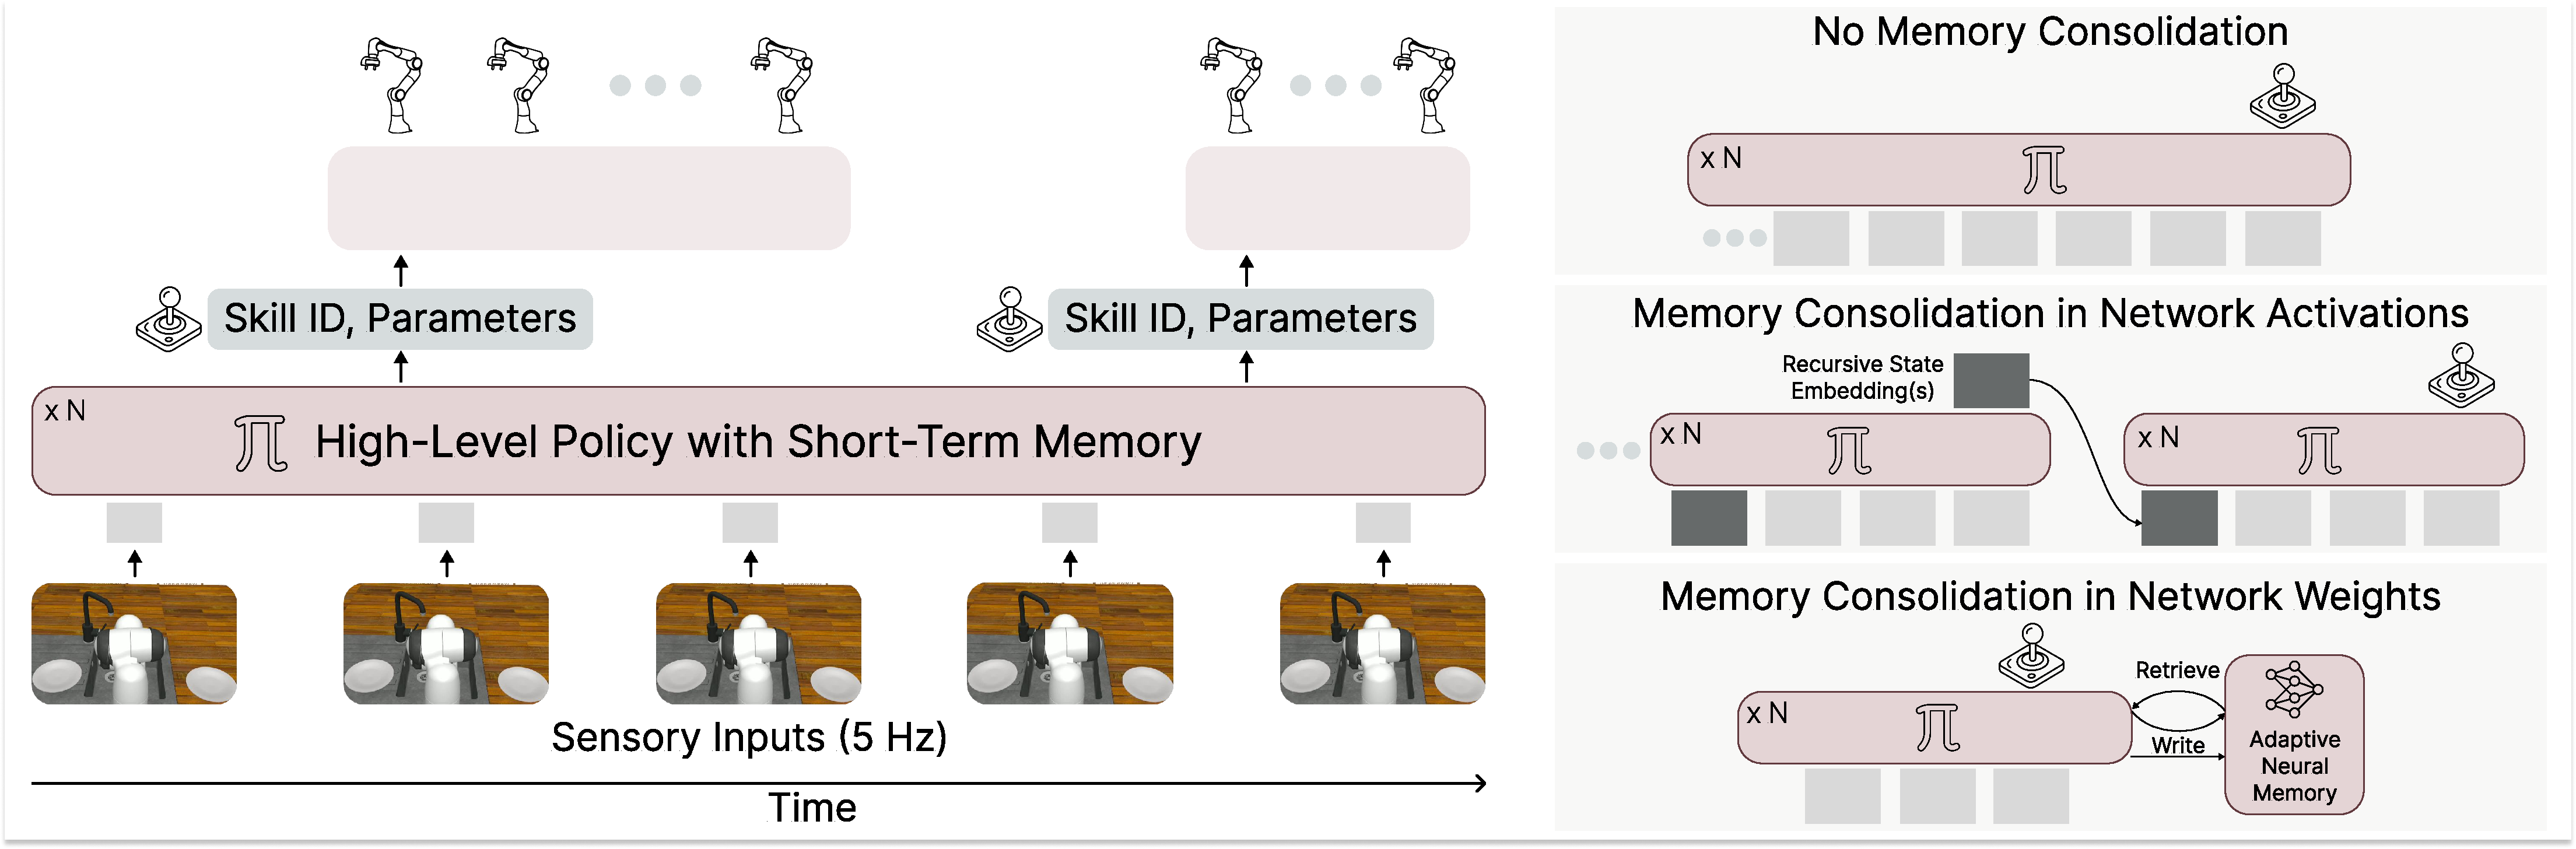
\includegraphics[width=0.9\linewidth]{figures/short-term-mem-diff.pdf}
  \caption{Proposed hierarchical architecture (left) with different high-level policy variants (right)}
  \label{fig:diff_arch}
\end{figure}

I propose that we should experiment with recent methods (See Fig.~\ref{fig:diff_arch}):   
\begin{itemize}[itemsep=2pt, topsep=0pt, parsep=0pt]
    \item No memory consolidation, e.g., transformers increasing context length
        \subitem Pros: No write policy; preserves fidelity
        \subitem Cons: Unbounded latency and memory; potentially noisy retrieval
    \item Online memory consolidation in activations, e.g., summary tokens
        \subitem Pros: Simple; bounded latency and memory
        \subitem Cons: Hard capacity bottleneck (depends on state dimension)
    \item Online memory consolidation in parameters, e.g., test-time training
        \subitem Pros: Strong compression; bounded latency and memory
        \subitem Cons: Harder optimization due to meta-training
\end{itemize}
\begin{tcolorbox}[clarifications]
\textbf{Clarification 1: Why is this called short-term memory?}
\\\\
The memory store is transient and resets at every episode.
\end{tcolorbox}

\section{Setup Description}
Overview
\begin{itemize}[itemsep=2pt, topsep=0pt, parsep=0pt]
    \item MAPLE with short-term memory--augmented high-level controller \( \pi_\theta \).
    \item  Hierarchical policy high-level controller \( \pi_\theta \) and skill library. The skill decides to pass the control back to \( \pi_\theta \) upon completion
    \item Real-world training: some demo-augmented reinforcement learning; some proof of concept for real-world execution is ``Practice Makes Perfect: Planning to Learn Skill Parameter Policies''
    \item Assumptions: Rewards for the task. Discrete skill parameters to reduce exploration space.
    % \item (Maybe) Real-world training: simulation pre-training + real-world finetuning of \( \pi_\theta \).
\end{itemize}
\paragraph{Policy}
\begin{itemize}[itemsep=2pt, topsep=2pt, leftmargin=12pt]
  \item \textbf{Hierarchical controller:} low-level skill library; the high-level policy selects the next skill and its parameters. After each skill completes, control returns to the high-level.
  \item \textbf{Adaptive within-episode memory:} augments the high-level policy; logs sensory inputs at $\sim$5\,Hz and retrieves them later via context-conditioned queries to inform decisions.
\end{itemize}

\paragraph{Task}
\begin{itemize}[itemsep=2pt, topsep=2pt, leftmargin=12pt]
  \item \textbf{Common task family} (e.g., cooking pasta) with controlled variants.
  \item \textbf{Memory probe (example):} salt is placed at one of $K$ candidate locations visible only in the initial frames; later success requires recalling that early sighting.
  \item \textbf{Extendable variants:} failure$\rightarrow$alternative plan, user-preference recall specified in language, and timer/prospective cues.
\end{itemize}

\paragraph{Training}
\begin{itemize}[itemsep=2pt, topsep=2pt, leftmargin=12pt]
  \item \textbf{End-to-end RL}, optionally bootstrapped with $\sim$5--20 expert demonstrations per variant for data efficiency.
  \item \textbf{Shared skill primitives} across variants; curriculum can scale episode length and number of distractors.
\end{itemize}

\paragraph{Evaluation}
\begin{enumerate}[itemsep=2pt, topsep=2pt, leftmargin=14pt]
  \item \textbf{Success rate} (primary).
  \item \textbf{Skill efficiency} (secondary): number of skills to completion; compare to an \emph{oracle skill budget} (ideal range under perfect memory).
\end{enumerate}